\chapter{Photonic Point-Gap Topology}
\label{ch:point-gap}

\begin{chapterlead}
The spectral winding number introduced in Chapter~\ref{ch:complex-bands}
counts how many times a complex band encircles a reference point. This
chapter specializes that invariant to photonic crystals with complex
permittivity, where the non-Hermiticity is rooted in the Maxwell
equations rather than in a tight-binding model. The discussion shows how reciprocity,
the vector nature of light, and the energy inner product constrain the
point-gap topology of photonic systems, derive the winding number from
a concrete one-dimensional setting, and connect the photonic winding
number to spectral flow, boundary accumulation, and the non-Bloch
bulk--boundary correspondence that have no analogue in the Hermitian
case.
\end{chapterlead}


%% ================================================================
\section{Point-gap topology from Maxwell Bloch states}
\label{sec:point-gap-maxwell}

In a one-dimensional photonic crystal with complex periodic permittivity
$\epsr(x) = \epsr(x + a)$, the Bloch eigenproblem
\begin{equation}
 -\left(\pdv{}{x} + ik\right)\frac{1}{\epsr(x)}
 \left(\pdv{}{x} + ik\right)\psi_k(x)
 = \frac{\omega(k)^2}{c^2}\,\psi_k(x)
 \label{eq:1d-bloch-complex}
\end{equation}
yields complex eigenfrequencies $\omega(k)$ for each Bloch wave vector
$k \in [-\pi/a, \pi/a]$. As $k$ sweeps the Brillouin zone, $\omega(k)$
traces a closed curve in the complex plane (closed because
$\omega(-\pi/a) = \omega(\pi/a)$ by periodicity).

If this curve does not pass through a reference point
$E_{\mathrm{ref}}$---typically chosen as zero or the center of the
spectral loop---the spectral winding number~\eqref{eq:winding-number}
is well defined and integer-valued~\cite{yao2018edge,yokomizo2019non,shen2017topological}. A nonzero winding number indicates
that the complex photonic band has a topologically nontrivial structure
that cannot be deformed to a point without closing the point gap.

\subsection{Maxwell-level origin}
\label{ssec:maxwell-origin}

The point-gap topology of the photonic band is not an artifact of a
tight-binding approximation---it is encoded directly in the Maxwell
operator. In the full Maxwell framework, the complex eigenfrequencies
arise because the operator
$\hat{\Theta}_k = -(d/dx + ik)\epsr^{-1}(d/dx + ik)$ is non-self-adjoint
when $\Im\epsr \neq 0$. The winding of the complex bands is a
spectral property of this continuous operator, not of a discretized
model.

The key Maxwell-level insight is that the \emph{shape} of the spectral
loop in the complex plane is determined by the spatial overlap between
the Bloch mode profile and the gain/loss distribution. Modes with
different $k$ sample the gain and loss regions differently, producing
different imaginary frequency shifts (Section~\ref{ssec:complex-bands-maxwell}).
The resulting $k$-dependent imaginary part creates the loop that winds
in the complex plane.

\begin{figure}[t]
 \centering
 
\includegraphics[width=0.72\textwidth]{fig_f13_complex_band_loop.pdf}
 \caption{A point gap is a hole in the complex spectrum, not a forbidden
 interval on the real axis. The asymmetric non-Hermitian loop winds
 around the reference point and cannot be contracted without crossing
 it; the reciprocal comparison curve collapses toward a non-winding
 real-line spectrum. The model is pedagogical, but the topology is the
 same integer winding used for complex photonic bands.}
 \label{fig:complex-band-loop}
\end{figure}

\begin{figure}[t]
 \centering
 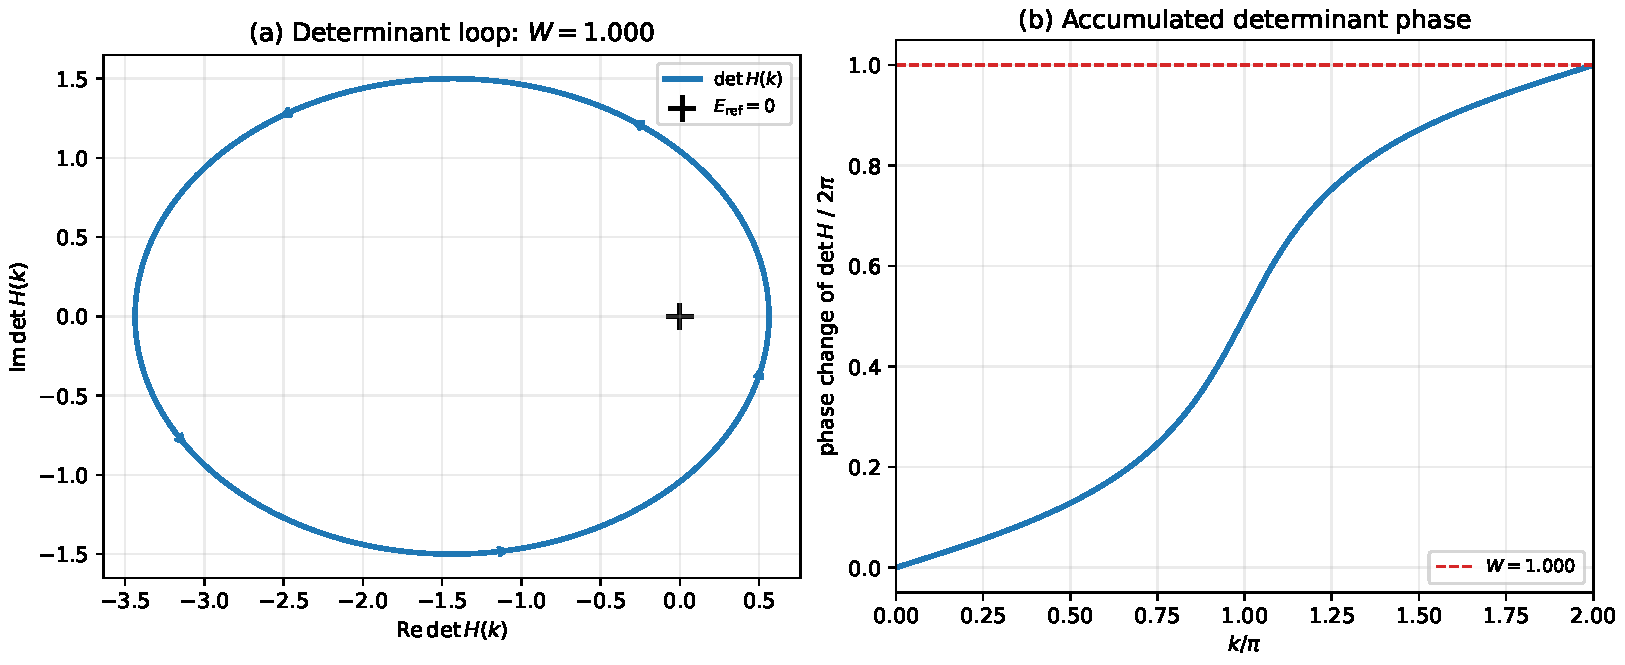
\includegraphics[width=0.85\linewidth]{figures/fig_f13_winding_number.pdf}
 \caption{Determinant winding for an asymmetric non-Hermitian SSH model
 ($t_L=1.75$, $t_R=0.25$, $t_2=1.0$). (a)~The loop traced by
 $\det H(k)$ winds once around the point-gap reference value
 $E_{\mathrm{ref}}=0$. (b)~The unwrapped phase of $\det H(k)$ changes
 by $2\pi$, giving $W=1.000000$. Computing the point-gap invariant from
 the determinant avoids branch ambiguities in square-root energy bands
 and matches the Maxwell-discretized form of the invariant.}
 \label{fig:determinant-winding}
\end{figure}

\subsection{Contrast with line-gap topology}
\label{ssec:line-vs-point}

It is instructive to contrast point-gap and line-gap topology. A
\emph{line gap} is a line in the complex plane (typically the real or
imaginary axis) that the spectrum does not cross. Line-gap topology
generalizes the Hermitian band-gap concept and supports the same
classification (Chern numbers, $\mathbb{Z}_2$ invariants) as Hermitian
systems. A \emph{point gap} is a single point that the spectrum does
not touch; the associated topology (the winding number) is purely
non-Hermitian and has no Hermitian counterpart.

For photonic systems, line-gap topology arises when the complex bands
are separated by a forbidden strip in the complex frequency plane---for
example, when gain and loss are weak enough that all bands remain close
to the real axis. Point-gap topology arises when the bands form loops
that encircle a reference energy---requiring stronger non-Hermiticity
that pushes the bands into genuinely two-dimensional curves in the
complex plane.


%% ================================================================
\section{Reciprocity constraints}
\label{sec:reciprocity-constraints}

Photonic systems are typically reciprocal (Section~\ref{sec:reciprocity}):
the permittivity tensor is symmetric, and the scattering matrix
satisfies $\Smat^\transpose = \Smat$. Reciprocity imposes a constraint
on the complex band structure: $\omega(k) = \omega(-k)$ for scalar
$\epsr$, because the Bloch Hamiltonian at $k$ and $-k$ is related by
transposition.

This constraint means the spectral loop $\omega(k)$ is symmetric under
$k \to -k$.  In one dimension, a reciprocal single-band spectral loop
necessarily retraces itself and carries zero winding, while a
multi-band determinant loop also retraces, forcing the total winding
number to vanish.  Breaking
reciprocity (e.g., with a magneto-optical component) lifts this
constraint and allows nonzero winding numbers~\cite{longhi2019probing,zhang2021observation,lin2023topological}.

\subsection{Reciprocity and vanishing point-gap winding}
\label{ssec:even-winding}

To see why reciprocity forces zero winding, write the spectral loop
as $\omega(k)$ for $k \in [-\pi/a, \pi/a]$.  Under $k \to -k$,
$\omega(-k) = \omega(k)$ (reciprocity).  The winding number
\begin{equation}
 \wnum = \frac{1}{2\pi i}\int_{-\pi/a}^{\pi/a}
 \frac{\omega'(k)}{\omega(k) - E_{\mathrm{ref}}}\;\dd k
 \label{eq:winding-integral}
\end{equation}
can be split into contributions $I_+$ (from $k \in [0,\pi/a]$) and
$I_-$ (from $k \in [-\pi/a,0]$).  Substituting $k \to -k$ in the
second integral, using $\omega(-k) = \omega(k)$ and
$\omega'(-k) = -\omega'(k)$, gives
\begin{equation}
 I_- = \frac{1}{2\pi i}\int_{0}^{\pi/a}
 \frac{-\omega'(k)}{\omega(k) - E_{\mathrm{ref}}}\;\dd k
 = -\,I_+.
 \label{eq:winding-cancellation}
\end{equation}
Therefore $\wnum = I_+ + I_- = 0$: the two half-Brillouin-zone
contributions cancel exactly.

In multi-band systems, the determinant
$\det[H(k) - E_{\mathrm{ref}}]$ also satisfies $k \to -k$ symmetry and
therefore retraces, giving zero total winding.  Individual eigenvalue
branches can still carry nonzero winding when they exchange partners at
symmetry-related $k$-points; such individual windings are constrained to
appear in cancelling pairs, so the sum vanishes.  Breaking
reciprocity---for example, with a magneto-optical
component---lifts this constraint and allows arbitrary integer
winding numbers~\cite{longhi2019probing,zhang2021observation,lin2023topological}.

\begin{booknote}[Why breaking reciprocity matters]
All one-dimensional photonic examples with nonzero point-gap winding
$\wnum \neq 0$ require broken reciprocity.  The Hatano--Nelson chain
(Chapter~\ref{ch:skin-effect}), the asymmetric SSH model, and
magneto-optical waveguide lattices all achieve $\wnum \neq 0$ precisely
because their Bloch Hamiltonians do not satisfy $H(-k)^{\mathrm{T}} = H(k)$.
In reciprocal systems, nontrivial topology protected by the transpose
symmetry can still exist, but it is classified by symmetry-protected
invariants (such as a $\mathbb{Z}_2$ index or a Pfaffian invariant)
rather than by the integer winding number $\wnum$ of the spectral
loop.  See the 38-fold classification in Chapter~\ref{ch:complex-bands}
for the full symmetry-resolved picture.
\end{booknote}

\subsection{Physical implications}
\label{ssec:even-winding-implications}

The vanishing of the ordinary reciprocal winding has concrete physical
consequences:
\begin{itemize}
 \item A reciprocal scalar 1D photonic crystal may have complex bands,
 exceptional points, or symmetry-protected non-Hermitian topology, but
 its ordinary determinant point-gap winding cancels between $k$ and
 $-k$.
 \item A nonzero integer winding in this 1D Maxwell setting normally
 requires a mechanism that makes forward and backward propagation
 inequivalent, such as magneto-optical bias, temporal modulation, or an
 engineered nonreciprocal reservoir.
 \item Breaking reciprocity (e.g., with a magneto-optical Faraday
 rotation element) allows odd winding numbers and the associated
 boundary spectral flow.
\end{itemize}

\begin{booknote}[Reciprocity and winding]
In tight-binding models, asymmetric hopping $t_L \neq t_R$ is a common
source of nonzero winding and the skin effect. In photonic crystals,
such asymmetry requires breaking reciprocity---a more demanding
experimental condition. Reciprocal photonic systems can still host
symmetry-protected non-Hermitian phases, but those phases should not be
identified with the ordinary integer winding of a single spectral loop.
The reciprocity constraint is a Maxwell-level selection rule that is
easy to miss in generic tight-binding models.
\end{booknote}


%% ================================================================
\section{Example: complex bands of a reciprocal bilayer}
\label{sec:nh-bilayer}

To make the abstract winding-number theory concrete, consider a
one-dimensional photonic crystal with period $a$ consisting of two
layers per unit cell:
\begin{itemize}
 \item Layer A: thickness $d_A = 0.5a$, index $n_A = 2.0 + 0.3i$
 (lossy).
 \item Layer B: thickness $d_B = 0.5a$, index $n_B = 2.0 - 0.1i$
 (gain, weaker than loss).
\end{itemize}
The gain and loss are \emph{not} balanced ($\PT$ symmetry is broken),
and the system is reciprocal. This example is useful because it shows
how complex photonic bands arise from Maxwell transfer matrices, but it
should not be mistaken for a nonzero point-gap winding phase: reciprocity
will make the ordinary Bloch loop retrace itself when the whole
Brillouin zone is followed.

\subsection{Transfer-matrix computation}
\label{ssec:bilayer-transfer}

The transfer matrix for one unit cell follows from the formalism of
Chapter~\ref{ch:periodicity}. Each layer contributes a propagation
matrix
\begin{equation}
 M_j = \begin{pmatrix}
 \cos\phi_j & -i\sin\phi_j/n_j \\
 -i\,n_j\sin\phi_j & \cos\phi_j
 \end{pmatrix},
 \qquad
 \phi_j = \frac{\omega\,n_j\,d_j}{c},
 \label{eq:complex-single-layer}
\end{equation}
and the full unit-cell matrix is $M = M_B\,M_A$. Because $n_j$ is now
complex, the phase $\phi_j$ has both real and imaginary parts:
$\phi_j = (\omega d_j/c)(\Re n_j + i\,\Im n_j)$. The imaginary part
causes exponential growth or decay within each layer, which is the
microscopic origin of the complex band structure.

The Bloch condition $\cos(Ka) = \xi(\omega) \equiv \tfrac{1}{2}\tr M$
generalises immediately: the half-trace $\xi$ is now complex, and the
Bloch wave vector $K$ is generically complex. For a fixed real~$k$,
the eigenfrequencies $\omega(k)$ are the solutions of
\begin{equation}
 \xi(\omega) = \cos(ka),
 \label{eq:bloch-condition-complex}
\end{equation}
which must be found numerically because the right-hand side is real
while $\xi(\omega)$ is an analytic function of $\omega$ in the complex
plane.

\paragraph{Numerical procedure.}
For each $k \in [-\pi/a, \pi/a]$, we solve
\eqref{eq:bloch-condition-complex} by Newton iteration in the complex
$\omega$ plane, initialising from the Hermitian band structure
($\Im n_j = 0$) and tracking the root as $\Im n_j$ is adiabatically
increased. With the parameters above ($n_A = 2.0 + 0.3i$,
$n_B = 2.0 - 0.1i$, $d_A = d_B = 0.5a$), the first band traces an
elliptical loop in the complex $\omega a/(2\pi c)$ plane with
centroid near $\Re\omega a/(2\pi c) \approx 0.22$ and an imaginary
spread of approximately $\pm 0.012$. The loop is tilted: the maximum
$\Im\omega$ occurs near $k = 0.3\pi/a$, not at the zone boundary,
because the mode profile at that wave vector has the largest spatial
overlap with the loss region.

The second band traces a separate loop at higher frequency. The two
loops do not intersect, confirming that the point gap between them is
well defined.

\subsection{Complex band structure}
\label{ssec:bilayer-bands}

Solving the Bloch condition numerically for $k \in [-\pi/a, \pi/a]$
yields complex eigenfrequencies $\omega(k)$. Over half of the Brillouin
zone the band can appear to form a non-circular arc in the complex
$\omega$ plane because layer A is lossier than layer B's gain. Over the
full Brillouin zone, however, the reciprocal partner at $-k$ retraces
the same spectral path. Thus the total determinant winding of this
reciprocal bilayer is zero, even though its bands are complex.

\subsection{Computing the winding number}
\label{ssec:winding-computation-ch13}

With the complex band $\omega(k)$ in hand, the spectral winding number
around a reference point $E_{\mathrm{ref}}$ is evaluated by discretising
the Brillouin zone into $N_k$ points $k_j = -\pi/a + 2\pi j/(N_k a)$
and summing the phase increments:
\begin{equation}
 \wnum = \frac{1}{2\pi}\sum_{j=0}^{N_k-1}
 \arg\!\left[
 \frac{\omega(k_{j+1}) - E_{\mathrm{ref}}}
 {\omega(k_j) - E_{\mathrm{ref}}}
 \right],
 \label{eq:discrete-winding}
\end{equation}
where $\arg$ returns a value in $(-\pi,\pi]$ and $k_{N_k} = k_0$
by periodicity. This formula is the discrete analogue
of~\eqref{eq:winding-integral}; it converges rapidly because the
spectral loop is smooth.

For the reciprocal bilayer, applying Eq.~\eqref{eq:discrete-winding} to
a single continuous band over the full Brillouin zone gives
$\wnum=0$ for any reference point not crossed by the spectrum. If one
artificially follows only half of the zone, or switches branches at a
degeneracy, an apparent winding can be obtained, but it is not the
integer point-gap invariant of the reciprocal Maxwell problem. A genuine
nonzero value requires replacing the bilayer by a nonreciprocal unit
cell so that the $k$ and $-k$ paths no longer cancel.

\begin{booknote}[Computational cost]
The bottleneck is solving~\eqref{eq:bloch-condition-complex} at each
$k_j$. For a 1D bilayer, this requires root-finding for a transcendental
equation---fast enough that the entire winding-number computation takes
milliseconds. For a 2D photonic crystal, the eigenproblem must be solved
by full-wave methods (Chapter~\ref{ch:numerics}), making the computation
substantially more expensive but still feasible with modern eigensolvers.
\end{booknote}

\subsection{Sensitivity to gain--loss contrast}
\label{ssec:bilayer-sensitivity}

As the imaginary parts of $n_A$ and $n_B$ are reduced toward zero, the
spectral loop contracts toward the real axis and eventually collapses to
a line segment (the Hermitian band structure). In the reciprocal
bilayer this contraction changes the shape of the complex band but not
the total point-gap winding, which remains zero. In a nonreciprocal
variant, by contrast, a winding transition would occur only when the
spectral path crosses the reference point and the point gap closes.

This point-gap closing is the non-Hermitian analogue of a Hermitian band
gap closing: the topological invariant can change only when the
reference point is touched by the spectrum.

Quantitatively, define a gain--loss parameter
$\gamma = \max(|\Im n_A|, |\Im n_B|)$ and fix
$\Im n_A/\Im n_B = -3$ (the ratio in our example). The critical
value $\gamma_c$ for a nonreciprocal winding transition depends on the
band gap of the underlying Hermitian structure: a larger Hermitian gap
requires a larger $\gamma_c$ to open a spectral loop wide enough to
wind. The reciprocal bilayer therefore serves as a useful warning:
large gain--loss contrast can create broad complex bands, but complex
bands alone do not imply a nonzero integer point-gap invariant.

\subsection{Relation to the Green's function}
\label{ssec:green-winding}

The point-gap winding number has an elegant reformulation in terms of
the retarded Green's function
$G(k,\omega) = [\omega^2/c^2 - \hat{\Theta}_k]^{-1}$.
At fixed reference frequency $E_{\mathrm{ref}}$, the winding can be
computed without tracking individual eigenvalues by following the phase
of the inverse Green's-function determinant across the Brillouin zone:
\begin{equation}
 \wnum(E_{\mathrm{ref}}) =
 \frac{1}{2\pi i}\int_{\mathrm{BZ}}
 \partial_k
 \ln\det\bigl[E_{\mathrm{ref}}^2/c^2 - \hat{\Theta}_k\bigr]\;\dd k,
 \label{eq:green-winding}
\end{equation}
provided the determinant never vanishes along the path. This connects
the point-gap topology directly to the analytic structure of the
photonic Green's function, which is the quantity measured in scattering
and emission experiments (Section~\ref{sec:point-gap-photonic}). In
practice, the resolvent formulation is useful for full-wave numerical
computations where the eigenfrequencies are not individually tracked but
the driven Maxwell problem can be solved at the reference frequency for
many values of $k$.


%% ================================================================
\section{From winding number to boundary response}
\label{sec:winding-to-edge}

The bulk-boundary correspondence for point-gap topology is subtler than
the Hermitian edge-state counting rule. A nonzero spectral winding of a
periodic one-dimensional system signals boundary-sensitive spectra:
under open boundary conditions the bulk eigenstates are generally
described by a generalized Brillouin zone and can accumulate near a
boundary through the non-Hermitian skin effect. The robust statement is
therefore not a simple counting formula such as
$N_{\mathrm{edge}}=|\wnum|$. Rather, the integer winding counts spectral
flow under a boundary twist and diagnoses the breakdown of the
conventional Bloch description.
This boundary response is qualitatively different from Chern edge modes
(Section~\ref{sec:bbc-hermitian}):
\begin{itemize}
 \item It can occur already in \emph{one-dimensional} systems, whereas
 Chern edge modes require at least two dimensions.
 \item It affects extensive bulk states as well as possible isolated
 defect or boundary resonances, reflecting the non-Hermitian skin
 effect (Chapter~\ref{ch:skin-effect}).
 \item It depends on the \emph{point gap}, not a line gap or a
 real-frequency band gap.
\end{itemize}

As Yao and Wang showed, the conventional Bloch-Hamiltonian winding can
give the wrong open-boundary prediction; the correct description uses
the \emph{generalized Brillouin zone} (Chapter~\ref{ch:skin-effect}).
The detailed mechanism by which the GBZ restores the bulk--boundary
correspondence is developed in Chapter~\ref{ch:bbc-rebuilt}.

\subsection{Spectral flow and parameter-driven transitions}
\label{ssec:spectral-flow}

The connection between winding number and boundary response can be
understood through spectral flow as a threading parameter is varied.
Consider a family of finite photonic systems parameterised by a twist angle
$\theta \in [0, 2\pi)$ applied as a boundary phase:
$\psi(x + La) = e^{i\theta}\psi(x)$. As $\theta$ sweeps from $0$
to $2\pi$, the finite-system eigenfrequencies trace paths in the
complex plane. The net number of eigenvalue trajectories that wind
around the reference point equals the point-gap winding $\wnum$---the
non-Hermitian analogue of the Laughlin spectral-flow argument.

This spectral flow provides an experimentally accessible probe of
point-gap topology: by threading a synthetic flux through a ring of
coupled resonators (equivalent to varying $\theta$), the movement of
resonance frequencies inside the point gap reveals the topological
invariant without computing the Bloch band structure.

\subsection{Boundary response of the bilayer}
\label{ssec:edge-bilayer}

For the reciprocal bilayer of Section~\ref{sec:nh-bilayer}, a finite
stack of $L$ unit cells with open (air) boundary conditions may support
surface resonances caused by impedance mismatch at the termination, but
these are not guaranteed by a nonzero point-gap winding because the
ordinary reciprocal winding vanishes. A nonreciprocal modification of
the same transfer-matrix model can instead produce a genuine skin
response. In that case, the bulk-mode decay length is set by the GBZ
radius deviation from unity:
\begin{equation}
 \xi_{\mathrm{skin}} \sim \frac{a}{|\ln r_{\mathrm{GBZ}}|},
 \label{eq:edge-localization}
\end{equation}
where $r_{\mathrm{GBZ}}$ is evaluated at the relevant complex
frequency. The distinction is important experimentally: observing a
localized resonance at a boundary is not by itself evidence for
point-gap topology. One must verify the boundary-sensitive spectral flow
or the non-Bloch displacement of the bulk spectrum.


%% ================================================================
\section{Two-dimensional point-gap topology}
\label{sec:2d-point-gap}

In two dimensions, point-gapped spectra have a new diagnostic absent in
one dimension: the periodic-boundary spectrum can cover a finite area in
the complex plane. The spectral-area result of Zhang, Yang, and
Fang~\cite{zhang2022universal} shows that this finite-area spectrum is
closely tied to geometry-dependent skin accumulation:
\begin{equation}
 \text{Spectral area} \neq 0
 \quad\Longrightarrow\quad
 \text{boundary-sensitive spectra in generic geometries}.
 \label{eq:spectral-area}
\end{equation}
The precise boundary response can depend on sample shape and symmetry,
so the spectral area should be read as a powerful diagnostic rather than
as a quantized invariant. It nevertheless explains why two-dimensional
non-Hermitian systems, including photonic crystal models with complex
$\epsr$, can show strong sensitivity to boundary conditions.

\subsection{Spectral area as a diagnostic}
\label{ssec:spectral-area-invariant}

For a single complex band $\omega(\kk)=x(\kk)+iy(\kk)$, a useful
oriented area with multiplicity is obtained from the Jacobian of the map
$\kk\mapsto (x,y)$:
\begin{equation}
 \mathcal{A} = \int_{\mathrm{BZ}}
 \left(\frac{\partial x}{\partial k_x}\frac{\partial y}{\partial k_y}
 - \frac{\partial x}{\partial k_y}\frac{\partial y}{\partial k_x}\right)
 \dd^2\kk
 = \int_{\mathrm{BZ}} J(\kk)\;\dd^2\kk,
 \label{eq:spectral-area-jacobian}
\end{equation}
where $J(\kk) \equiv \partial(x, y)/\partial(k_x, k_y)$ is the
Jacobian of the map $\kk \mapsto \omega(\kk)$ from the 2D Brillouin
zone to the complex energy plane. This Jacobian measures how much
oriented spectral area the band map creates locally. If $J$ has a fixed
sign, the map is orientation-preserving and the projected spectrum
covers a finite area; if $J$ changes sign, different regions of the BZ
can cancel in the oriented integral. The physical, unsigned area of the
spectral image is not generally quantized and must be interpreted with
this multiplicity caveat.

Equivalently,
\begin{equation}
 J(\kk) = 2\,\Im\!\left[
 \frac{\partial \omega_n}{\partial k_x}
 \frac{\partial \bar{\omega}_n}{\partial k_y}\right]
 = 2\left(
 \frac{\partial \Re\,\omega_n}{\partial k_x}
 \frac{\partial \Im\,\omega_n}{\partial k_y}
 - \frac{\partial \Re\,\omega_n}{\partial k_y}
 \frac{\partial \Im\,\omega_n}{\partial k_x}
 \right).
 \label{eq:jacobian-berry}
\end{equation}
This expression shows that spectral area requires the real and
imaginary parts of the eigenfrequency to vary independently across the
BZ---a hallmark of genuine non-Hermiticity, as opposed to a uniform
global loss that merely shifts all eigenvalues by a constant imaginary
offset.

\paragraph{Example: filled spectral disk.}
For a model whose two-dimensional Brillouin zone maps once onto a disk
of radius $R$ centred at $\omega_0$ in the complex plane, the unsigned
spectral area is
\begin{equation}
 \mathcal{A} = \pi R^2.
 \label{eq:circular-area}
\end{equation}
If the map covers the same disk several times with the same orientation,
the oriented area counts the multiplicity. Figure~\ref{fig:spectral-area}
illustrates the corresponding spectral image for a 2D lattice model.

This area is not a quantized topological invariant. A nonzero spectral
area instead serves as a practical diagnostic, and in generic settings a
strong indicator, of non-Hermitian boundary sensitivity in two
dimensions.

\subsection{Implications for photonic crystals}
\label{ssec:2d-photonic}

For a two-dimensional photonic crystal with complex $\epsr(\rr)$, the
PBC band structure can cover a finite area in the complex $\omega$
plane. The practical consequences are far-reaching. First, the PBC band
structure is
\emph{not} a reliable guide to the physics of a finite sample: the
eigenfrequencies of a finite photonic crystal slab can differ
qualitatively from the PBC bands, with extensive piling up of modes
near selected boundaries. Second, conventional edge or corner resonances
must be distinguished from non-Hermitian boundary accumulation using
non-Bloch theory rather than ordinary Bloch invariants. Third, the
spectral area itself can be computed efficiently from the PBC band
structure using~\eqref{eq:spectral-area-jacobian} on a discrete
$\kk$-grid, providing a practical diagnostic for boundary sensitivity in
a given 2D photonic crystal design.

\paragraph{Example: lossy square-lattice rods.}
Consider a square array of dielectric rods ($\varepsilon = 12 + 0.4i$,
radius $r = 0.2a$) in air. For TM polarization, the first band at
$\kk = (k_x, k_y)$ sweeps a closed surface in the three-dimensional
space $(\Re\omega, \Im\omega, k_x, k_y)$. Projected onto the complex
$\omega$ plane, the band covers an area
$\mathcal{A} \sim 0.003\,(2\pi c/a)^2$. Although this area is small,
it is nonzero, so the finite rod array should be checked for
boundary-sensitive spectra and possible skin accumulation. The direction
and strength of the accumulation depend on the detailed termination and
on the effective imaginary gauge field.

In practice, the skin effect in 2D photonic crystals is weaker and
harder to observe than in 1D because the spectral area scales with the
imaginary part of $\varepsilon$ and the group velocity, both of which
are modest for typical photonic-crystal parameters. Corner modes
associated with second-order point-gap topology have been predicted
theoretically but remain experimentally elusive.

\paragraph{Higher-order point-gap topology.}
In two dimensions, the point-gap classification admits a
$\mathbb{Z}$-valued second-order invariant that predicts corner-localised
modes in systems with spatial symmetries. For a photonic crystal with
$C_4$ symmetry and complex $\epsr$, the corner invariant is the
symmetry indicator or nested non-Bloch winding defined in the appropriate
generalized Brillouin zone. This higher-order topology is the
non-Hermitian analogue of the quadrupole topological insulator, but its
photonic realization requires more than gain/loss: the relevant spatial
symmetry and the non-Bloch boundary spectrum must both be verified.


%% ================================================================
\section{Photonic realizations and experiments}
\label{sec:point-gap-photonic}

Point-gap topology and the related skin response have been proposed and
observed in wave platforms including photonic analogues~\cite{he2016acoustic,yuan2025breakdown}:

\begin{figure}[t]
 \centering
 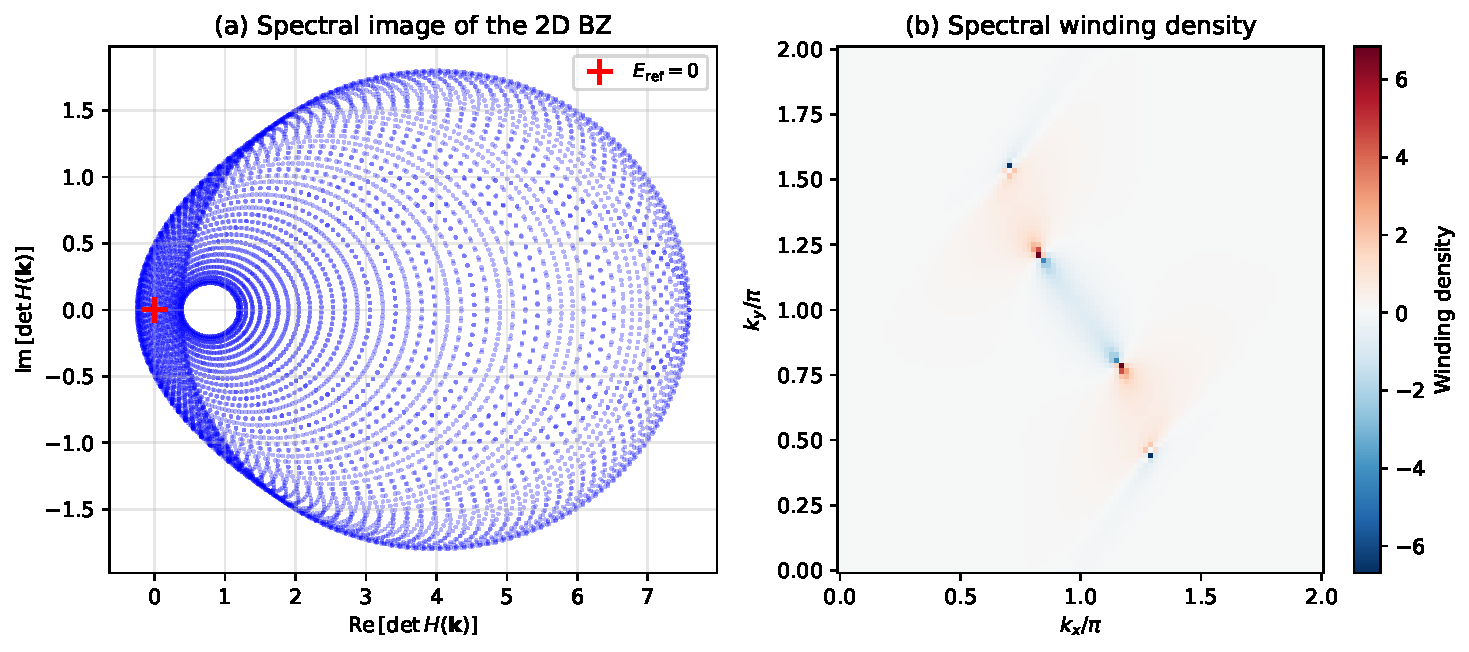
\includegraphics[width=0.85\linewidth]{figures/fig_f13_spectral_area.pdf}
 \caption{Spectral image of the 2D BZ for a non-Hermitian lattice model
 ($t_L = 1.5$, $t_R = 0.5$, $t_2 = 1.0$, $t_3 = 0.8$).
 (a)~The function $\det H(\kk)$ maps the 2D Brillouin zone into the
 complex plane (blue dots); the reference point $E_{\mathrm{ref}} = 0$
 (red cross) lies inside the image. This signals boundary sensitivity
 but is not by itself an integer edge-state count.
 (b)~Jacobian density across the BZ, showing where the map locally
 creates positive or negative oriented area. The total spectral area
 $A \approx 4.7$ is a diagnostic of non-Hermitian boundary response.}
 \label{fig:spectral-area}
\end{figure}

\paragraph{Coupled-resonator arrays.}
Chains of microring resonators with asymmetric coupling (via auxiliary
gain/loss elements) realize the non-Hermitian SSH model with tunable
winding numbers. The asymmetry can be introduced by gain/loss-induced
effective non-reciprocal coupling or by auxiliary waveguide paths that
create direction-dependent hopping. The winding number has been inferred
from the spectral sensitivity to boundary conditions and from the direct
observation of skin-mode localization.

\paragraph{Photonic lattices with on-site gain/loss.}
Arrays of waveguides with alternating gain and loss can exhibit point-gap
topology when the gain/loss pattern is combined with a mechanism that
breaks the cancellation between forward and backward propagation. In
these systems, the winding number can be tuned by varying the pump
intensity, providing a continuous knob for controlling the topological
phase.

\paragraph{Non-reciprocal photonic crystals.}
Magneto-optical photonic crystals provide a natural platform for odd
winding numbers, connecting point-gap topology to the anomalous photonic
Hall effect. These systems require an external magnetic field but offer
the largest topological gaps and the strongest skin-effect localization.

\paragraph{Photonic-crystal point-gap observation.}
Zhong et al.~\cite{zhong2021non} proposed and analyzed a concrete
photonic-crystal model with non-Hermitian point-gap topology, computing
the spectral winding number from the complex photonic band structure and
demonstrating its connection to boundary-sensitive spectra and the skin
effect. Their analysis shows that the point-gap invariant can be
extracted from full-wave electromagnetic simulations, establishing a
direct link between the abstract topological theory and realistic
photonic structures.


%% ================================================================
\section{Vector nature and polarization}
\label{sec:vector-point-gap}

In two and three dimensions, the vector nature of the electromagnetic
field introduces additional structure. Each Bloch band carries a
polarization (TE, TM, or mixed), and the point-gap winding can depend on
the polarization sector. For a 2D photonic crystal slab:
\begin{itemize}
 \item TE-like and TM-like bands can have different winding numbers,
 leading to polarization-dependent skin effects.
 \item Band crossings between TE and TM sectors can create exceptional
 points that connect the point-gap topology to the EP topology of
 Chapter~\ref{ch:exceptional-points}.
 \item The full vectorial Maxwell calculation is essential for
 quantitative predictions; scalar approximations can give the wrong
 winding number.
\end{itemize}

This polarization dependence is a uniquely photonic feature with no
analogue in scalar wave systems or electronic topological insulators.

\paragraph{Polarization-resolved winding.}
In a concrete 2D photonic crystal slab, the TE-like and TM-like bands
generally have different spatial profiles: the TM modes concentrate their
electric field inside the high-index rods, while the TE modes spread
into the air region. When $\Im\epsr$ is nonzero only inside the rods,
the TM bands acquire larger imaginary frequency shifts and trace wider
loops in the complex plane, potentially reaching a higher winding number
than the TE bands. The resulting polarisation-dependent skin effect
means that a finite photonic-crystal slab can localise TM light at one
boundary while TE light remains extended---a polarisation filter driven
entirely by non-Hermitian topology.

\paragraph{From scalar to vector: when does the winding change?}
A useful rule of thumb is that the scalar (single-polarisation)
winding number agrees with the full vectorial result whenever
the TE--TM coupling is negligible---i.e., when the photonic crystal has
a mirror symmetry that decouples the polarisations. When this symmetry
is broken (e.g., by a tilted slab, an anisotropic $\epsr$ tensor, or
a substrate), the TE and TM bands hybridise, and the winding number of
the hybridised band can differ from the sum of the individual
polarisation windings. In the extreme case of an exceptional-point
degeneracy between TE and TM bands, the winding number changes by
$\pm 1$, connecting the point-gap topology directly to the EP
classification of Chapter~\ref{ch:exceptional-points}.


\begin{takeaway}[Point-gap topology is intrinsically non-Hermitian]
Point-gap topology has no Hermitian analogue: a real-valued spectrum
cannot wind around a point in the complex plane. In photonic systems,
it arises from the interplay of complex $\epsr$, spatial periodicity,
and (optionally broken) reciprocity. The Maxwell-level constraint of
reciprocity cancels the ordinary one-dimensional determinant winding,
so genuine integer point-gap winding in photonic systems usually
requires nonreciprocity or a symmetry-resolved invariant. The physical
manifestation of point-gap topology---boundary-sensitive spectra and
the non-Hermitian skin effect---is the subject of
Chapter~\ref{ch:skin-effect}, and the rebuilt bulk-boundary
correspondence that accounts for it is developed in
Chapter~\ref{ch:bbc-rebuilt}.
\end{takeaway}
